\documentclass[preprint]{aastex}
%\documentclass{emulateapj}


% has to be before amssymb it seems
%\usepackage{color,hyperref}
%\definecolor{linkcolor}{rgb}{0,0,0.5}
%\hypersetup{colorlinks=true,linkcolor=linkcolor,citecolor=linkcolor,
%            filecolor=linkcolor,urlcolor=linkcolor}
%\usepackage{amssymb,amsmath}

\usepackage{color}
\usepackage{url}
\usepackage{graphicx}
\graphicspath{{figures/}}

% For Python code
\usepackage{listings}
\definecolor{lbcolor}{rgb}{0.9,0.9,0.9}
\lstset{language=Python,
        basicstyle=\footnotesize\ttfamily,
        showspaces=false,
        showstringspaces=false,
        tabsize=2,
        breaklines=false,
        breakatwhitespace=true,
        identifierstyle=\ttfamily,
        keywordstyle=\bfseries\color[rgb]{0.133,0.545,0.133},
        commentstyle=\color[rgb]{0.133,0.545,0.133},
        stringstyle=\color[rgb]{0.627,0.126,0.941},
    }

% Draft watermark:
%\usepackage{draftwatermark}
%\SetWatermarkLightness{0.9}
%\SetWatermarkScale{4}

\usepackage{amsmath}
\DeclareMathOperator{\sinc}{sinc}
\DeclareMathOperator{\III}{III}

% Some macros
\newcommand{\todo}[1]{{\color{red} [TODO: #1]}}
\newcommand{\foreign}[1]{{\it #1}}

\newcommand{\apriori}{\foreign{a priori}}
\newcommand{\adhoc}{\foreign{ad hoc}}
\newcommand{\etal}{\foreign{et\,al.}}
\newcommand{\etc}{\foreign{etc.}}

\newcommand{\Fig}[1]{Figure~\ref{fig:#1}}
\newcommand{\fig}[1]{\Fig{#1}}
\newcommand{\figlabel}[1]{\label{fig:#1}}
\newcommand{\Eq}[1]{Equation~(\ref{eq:#1})}
\newcommand{\eq}[1]{\Eq{#1}}
\newcommand{\eqs}[2]{Equations~(\ref{eq:#1})-(\ref{eq:#2})}
\newcommand{\eqlabel}[1]{\label{eq:#1}}
\newcommand{\Sect}[1]{Section~\ref{sect:#1}}
\newcommand{\sect}[1]{\Sect{#1}}
\newcommand{\sects}[1]{Sections~#1}
\newcommand{\App}[1]{Appendix~\ref{sect:#1}}
\newcommand{\app}[1]{\App{#1}}
\newcommand{\sectlabel}[1]{\label{sect:#1}}

\usepackage[normalem]{ulem}
\newcommand{\new}[1]{{\color{red} #1}}
\newcommand{\old}[1]{{\sout{#1}}}


\begin{document}

\title{Practical Considerations for Lomb-Scargle Periodic Analysis}

\newcommand{\escience}{*}
\newcommand{\uwastro}{+}
\author{Jacob T. VanderPlas\altaffilmark{\escience}}
\altaffiltext{\escience}{eScience Institute, University of Washington}


\begin{abstract}
An introduction to practical aspects of the use of Lomb-Scargle-type algorithms for periodic analysis.
\end{abstract}

\keywords{
    methods: data analysis ---
    methods: statistical
}

\section{Introduction}
\sectlabel{introduction}

\begin{figure}[ht]
\centering
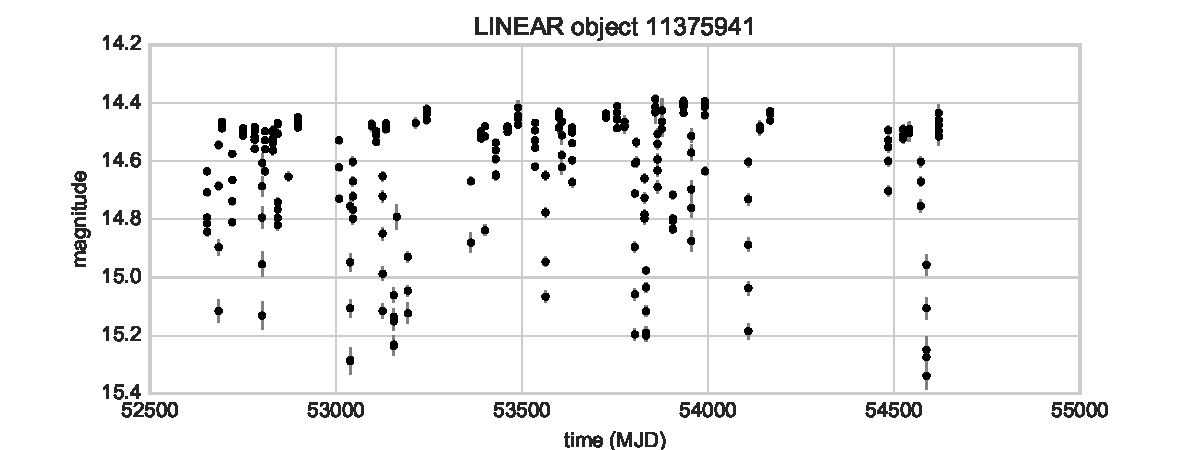
\includegraphics[width=\textwidth]{fig01_LINEAR_data}
\caption{Observed light curve from LINEAR object ID 11375941
    \figlabel{LINEAR_data}.
}
\end{figure}


\begin{figure}[ht]
\centering
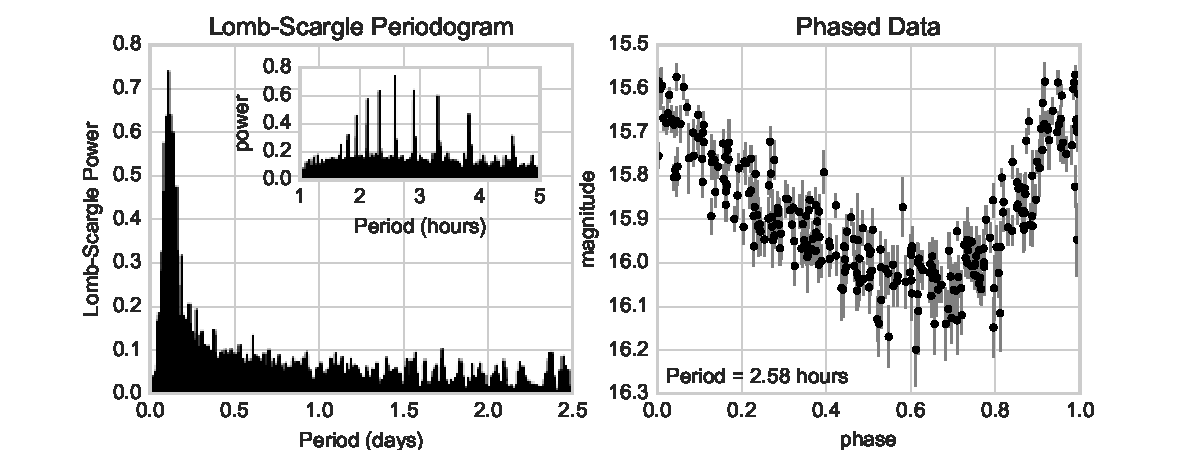
\includegraphics[width=\textwidth]{fig02_LINEAR_PSD}
\caption{{\it Left panel:} the Lomb-Scargle periodogram computed from the data
    shown in \fig{LINEAR_data}, with an inset detailing the interesting region.
    {\it Right panel:} the input data in \fig{LINEAR_data}, folded over the
    2.58-hour period to show the coherent periodic variability.
    \figlabel{LINEAR_power}
}
\end{figure}

The Lomb-Scargle periodogram \citep{Lomb76, Scargle82}
is a well-known algorithm for detecting periodicity
in unevenly-sampled time-series, particularly within the astronomy community.
For example, consider the data shown in \fig{LINEAR_data}.
This is an irregularly-sampled timeseries showing a single object from the
LINEAR survey, with magnitude measured 280 times over the course of five and
a half years.

By eye, it is clear that the brightness of the object varies in time with a range spanning approximately 0.8 magnitudes, but what is not immediately clear is that this variation is periodic in time.
The Lomb-Scargle periodogram is a method that allows efficient computation of a Fourier-like power spectrum from such unevenly-sampled data, resulting in an intuitive means of determining the period of oscillation.

The left panel of \fig{LINEAR_power} shows the Lomb-Scargle periodogram computed for the data in \fig{LINEAR_data}
Computing the Lomb-Scargle periodogram for the data gives us a measure of the
power as a function of period of oscillation (\fig{LINEAR_power}, left), from
which we can determine the period of oscillation of approximately 2.58 hours.
The right panel of \fig{LINEAR_power} shows a folded visualization of
the same data as \fig{LINEAR_data} -- i.e.{} plotted as a function of phase
rather than time.\footnote{
    The periodogram in \fig{LINEAR_power}was computed using
    {\tt astropy.stats.LombScargle}
    from the AstroPy project \citep{Astropy2013};
    Python code to reproduce this figure is available at
    \url{http://github.com/jakevdp/PracticalLombScargle/}
}

Often this is exactly how the Lomb-Scargle periodogram is presented: as a clean, well-defined procedure to detect the periodic component in an unevenly-sampled dataset.
In practice, however, there are a number of subtle issues that must be considered when applying a Lomb-Scargle analysis to real-world datasets, and I have found that these are rarely presented together at an introductory level.
This paper seeks to fill that gap, and provide a practical, semi-technical guide to the effective use of the Lomb-Scargle method of periodic analysis.
This paper does not seek a complete or rigorous treatment of the mathematics involved, but rather seeks to develop the intuition of {\it how} to think about the issues involved.


\section{Background: the Continuous Fourier Transform}

In order to understand how we should interpret the Lomb-Scargle periodogram, we will first briefly step back and review the subject of Fourier analysis of continuous signals.
Consider a continuously-defined signal $g(t)$.
Its Fourier transform is given by the following integral:
\begin{equation}
    \hat{g}(f) \equiv \int_{-\infty}^\infty g(t) e^{-2\pi i f t} dt
    \eqlabel{FT-def}
\end{equation}
The inverse relationship is given by:
\begin{equation}
    g(t) \equiv \int_{-\infty}^\infty \hat{g}(f) e^{+2\pi i f t} df
    \eqlabel{IFT-def}
\end{equation}
For convenience we will also define the Fourier transform operator
$\mathcal{F}$, such that
\begin{eqnarray}
    \mathcal{F}\{g\} &=& \hat{g} \\
    \mathcal{F}^{-1}\{\hat{g}\} &=& g
\end{eqnarray}

The continuous Fourier transform has a number of useful properties that we will make use of in our discussion.

\begin{description}
   \item[The Fourier transform is a linear operation.]
     That is, for any constant $A$ and any functions $f$ and $g$, we can write
     \begin{eqnarray}
       \mathcal{F}\{f(t) + g(t)\} &=& \mathcal{F}\{f(t)\} + \mathcal{F}\{g(t)\}\nonumber\\
       \mathcal{F}\{A f(t)\} &=& A\mathcal{F}\{f(t)\},
     \end{eqnarray}
     which follows from the linearity of the Fourier integral.

   \item[The Fourier transform of sinusoid with frequency $f_0$ is a sum of delta functions at $\pm f_0$.]
     Given the integral definition of the Dirac delta function, it is straightforward to show that
     \begin{equation}
       \mathcal{F}\{e^{2\pi f_0 t}\} = \delta(f - f_0).
       \eqlabel{delta_FT}
     \end{equation}
     Euler's formula shows how such a complex exponential
     can be expressed in terms of sines and cosines:
     \begin{equation}
       e^{2\pi f_0 t} = \cos(2\pi f_0 t) + i\sin(2\pi f_0 t).
       \eqlabel{Euler_formula}
     \end{equation}
     Using the linearity of the Fourier transform, we can take these identites
     and derive the following:
     \begin{eqnarray}
       \mathcal{F}\{\cos(2\pi f_0 t)\} &=& \frac{1}{2}\left[\delta(f - f_0) + \delta(f + f_0)\right]\\
       \mathcal{F}\{\sin(2\pi f_0 t)\} &=& \frac{1}{2i}\left[\delta(f - f_0) - \delta(f + f_0)\right].
     \end{eqnarray}
     In other words, a sinusoidal signal with frequency $f_0$ has a Fourier transform consisting of a weighted sum of delta functions at $\pm f_0$.

   \item[A time-shift imparts a phase in the Fourier transform.]
     In other words, for any well-behaved function $g(t)$ we can write
     \begin{equation}
       \mathcal{F}\{g(t - t_0)\} = \mathcal{F}\{g(t)\} e^{-2\pi i ft_0}
     \end{equation}
     The key observation here is that the time-shift does not change the
     amplitude of the resulting transform, but only the phase.
\end{description}

These properties taken together make the Fourier transform quite useful for the study of periodic signals.
The linearity of the transform means that any signal made up of a sum of periodic components will have a Fourier transform consisting of a sum of delta functions at those frequencies: that is, the Fourier transform is a {\it direct} measure of the periodic content of a function.

Further, if we compute the squared amplitude of the resulting transform, we can both do away with complex components and remove the phase imparted by any time offsets; this squared amplitude is usually known as the {\it Power Spectrum}:
\begin{equation}
  \mathcal{P}\{g\} \equiv \left|\mathcal{F}\{g\}\right|^2
\end{equation}
The power spectrum of a function is a positive real-valued function of $f$ that quantifies the contribution of each frequency $f$ to the total signal.

\subsection{Some Useful Fourier Pairs}

\begin{figure}[ht]
\centering
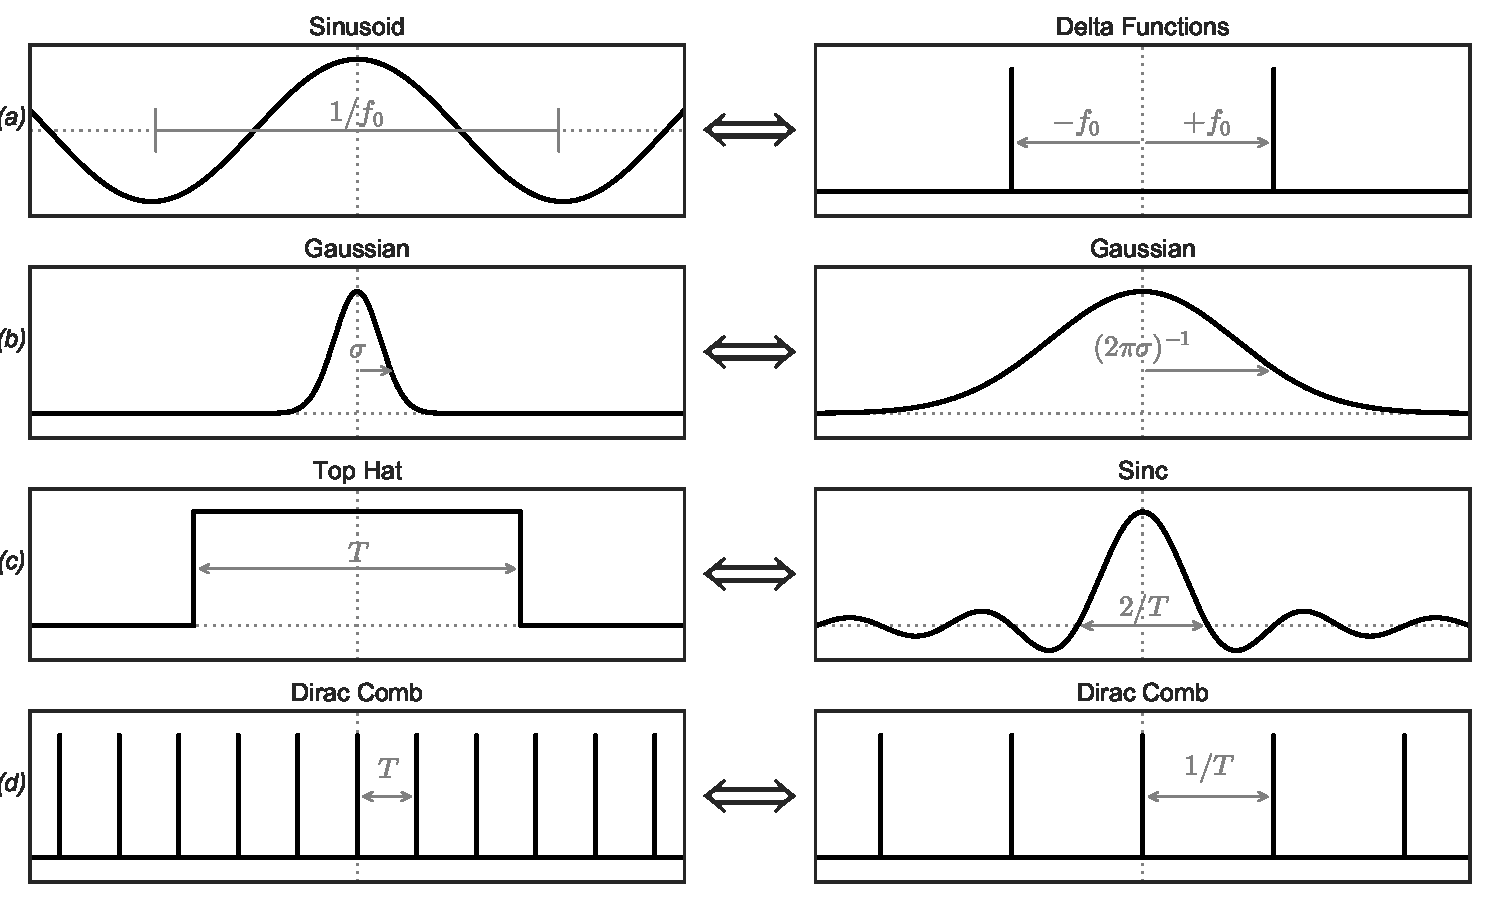
\includegraphics[width=\textwidth]{fig03_Fourier_pairs}
\caption{Visualization of important Fourier pairs.\figlabel{fourier_pairs}}
\end{figure}

We have already discussed that the Fourier transform of a complex exponential is a single delta function.
This is just one of many ``Fourier Pairs'' to keep in mind as we progress to understanding the Lomb-Scargle Periodogram.
We list a few more important pairs here (see \Fig{fourier_pairs} for a visual representation of the following pairs):


\begin{description}
  \item[The Fourier transform of a sinusoid is a pair of Delta functions.]
    \begin{equation}
      \mathcal{F}\{\cos(2\pi f_0 t)\} = \frac{1}{2}\left[\delta(f-f_0) + \delta(f+f_0)\right]
    \end{equation}
    We saw this above, but repeat it here for completeness.

   \item[The Fourier transform of a Gaussian is a Gaussian.]
     \begin{equation}
       \mathcal{F}\{{\rm N}(t; \sigma)\} = \frac{1}{\sqrt{2\pi\sigma^2}}{\rm N}\left(f;\frac{1}{2\pi\sigma}\right)
     \end{equation}
     The Gaussian function ${\rm N}(t, \sigma)$ is given by
     \begin{equation}
       {\rm N}(t; \sigma) \equiv \frac{1}{\sqrt{2\pi\sigma^2}}e^{-t^2 / (2\sigma^2)}
     \end{equation}

  \item[The Fourier transform of a tophat function is a sinc function.]
    \begin{equation}
      \mathcal{F}\{\Pi_T(t)\} = \sinc(f T)
    \end{equation}
    The tophat function, $\Pi_T(t)$ is a normalized symmetric function that
    is uniform within a range given by $T$, and zero elsewhere:
    \begin{equation}
      \Pi_T(t)  \equiv \left\{
      \begin{array}{ll}
        1 / T, & |t| \le T / 2 \\
        0,     & |t| > T / 2
      \end{array}
      \right.
    \end{equation}
    The sinc function is given by the standard definition:
    \begin{equation}
      \sinc(x) \equiv \frac{\sin(\pi x)}{\pi x}
    \end{equation}

  \item[The Fourier transform of a Dirac comb is a Dirac comb.]
    \begin{equation}
      \mathcal{F}\{\III_T(t)\} = \frac{1}{T}\III_{1/T}(f)
    \end{equation}
    The Dirac comb $\III_T(t)$ is an infinite sequence of Dirac delta functions
    placed at even intervals of size $T$:
    \begin{equation}
      \III_T(t) \equiv \sum_{k=-\infty}^\infty \delta(t - kT)
    \end{equation}
\end{description}

The key observation in each of these is the reciprocity of scales across the
Fourier transform: a function with a characteristic scale $T$ will generally
have a Fourier transform with characteristic scale proportional to $1/T$.
This feature will turn out to be very important as we push further in
understanding the Lomb-Scargle Periodogram.

\subsection{Windowing and Convolution}

\begin{itemize}
  \item mention convolution theorem; show how it leads to windowing
  \item figure: show how windowing works
\end{itemize}


\section{From Continuous to Discrete Signals}

\begin{itemize}
  \item discrete signal as a Dirac comb window
  \item derive the Nyquist limit from the Dirac comb FT
  \item derive the Schuster periodogram
  \item mention the FFT
\end{itemize}


\section{Non-uniform sampling}

\begin{itemize}
  \item nonuniform signal as sum-of-deltas window function
  \item Nyquist limit does not exist!
  \item 
\end{itemize}


\section{The Lomb-Scargle Periodogram}

\begin{itemize}
  \item Show relation to Schuster periodogram
  \item Show relation to least squares fitting of sinusoid
  \item Key: LS measures {\it windowed} power spectrum
  \item Show effects of truely random sampling; of Kepler-like sampling; of ground-based nightly sampling
\end{itemize}


\section{Using Lomb-Scargle Effectively}

\begin{itemize}
  \item Frequency grid
  \item Peak width
\end{itemize}


\subsection{Uncertainties in Periods}

\begin{itemize}
  \item Peak Width
  \item False Alarm Probability and why it fails
  \item Baluev method and why it's not enough
  \item Boostrap

\end{itemize}



\section{Algorithmic Considerations}

\begin{itemize}
\item Press \& Rybicki method; show some benchmarks.
\item NFFT method
\end{itemize}



\section{Generalizations \& Challenges}

\begin{itemize}
\item Bayesian view doesn't make sense
\item Multiterm makes the true period fit better, but also bumps the background noise.
\end{itemize}




\newpage

\section{Draft stuff below...}

\begin{itemize}
    \item transform and inverse
    \item properties (delta function $\to$ sinusoid, time shift $\to$ phase, convolution theorem)
    \item motivating the power spectrum
    \item some important Fourier pairs (sinusoid$\to$delta, dirac comb$\to$dirac comb, Gaussian$\to$gaussian, top-hat$\to$sinc)
\end{itemize}

\subsection{Motivating the Power Spectral Density}

If you explore the properties of the Fourier transform, you will discover
a couple important properties:

\begin{description}
\item[The Fourier Transform is a Linear Operation.]
This means that for functions $a$ and $b$ and scalar $A$,
\begin{eqnarray}
    \mathcal{F}(a + b) &=& \mathcal{F}(a) + \mathcal{F}(b) \\
    \mathcal{F}(A \cdot a) &=& A\cdot\mathcal{F}(a).
\end{eqnarray}
These properties follow straightforwardly from the linearity of integration.
\item[The Fourier Transform of a Sinusoid with frequency $f_0$ is a pair of delta
      functions at $\pm f_0$.]
    That is, if $g(t) = \sin(2\pi f_0 t)$, then
    \begin{equation}
        \hat{g}(f) = \frac{i}{2} \bigg(\delta(f - f_0) - \delta(f + f_0) \bigg)
    \end{equation}
    This can be shown straightforwardly using Euler's formula and the integral
    definition of the Dirac delta function.
\item[The Fourier Transform of a time-shifted function is unchanged up to a phase.]
    That is, if $g_\tau(t) = g(t - \tau)$, then
    \begin{equation}
        \hat{g}_\tau(f) = \phi(\tau)\hat{g}(f)
    \end{equation}
    where $\phi$ is a phase that depends on the time-shift $\tau$.
    This can be confirmed via a change of variables in \eq{FT-def}.
\end{description}
These properties are central to the well-known ability of the Fourier transform
to measure frequency information from a continuous signal: a signal
with a periodic component at frequency $f_0$ will have a Fourier transform
reflecting that frequency. Moreover, we can remove the effect of the phase by
taking the squared magnitude of the Fourier transform; this is the power
spectral density:
\begin{equation}
    \mathcal{P}(g) \equiv \left|\mathcal{F}(g)\right|^2
\end{equation}
Because this operation removes the phase, we now have a quantity that is
{\it insensitive to time-shifts} and consists of a
{\it delta function for each sinusoidal frequency within the data}.
If we want to detect periodic components in a continuous signal,
this will be a very useful quantity.

\subsection{Other Identities}

\begin{description}
\item[Convolution Theorem.]
    The convolution theorem states that the
    Fourier transform of a convolution is a product of the Fourier transforms:
    \begin{equation}
      \mathcal{F}\{g \ast h\} = \mathcal{F}\{g\}\mathcal{F}\{h\}
    \end{equation}
    where the convlution operator $\ast$ is defined by
    \begin{equation}
      \{g \ast h\}(t) \equiv \int_{-\infty}^\infty g(t - \tau) h(\tau) d\tau.
    \end{equation}
    This can be confirmed via the linearity of integration and the integral
    definition of the Dirac delta function.
\item[The Fourier Transform of a Gaussian is a Gaussian.]
    The Gaussian function is defined as
    \begin{equation}
    G(t;\sigma) \propto \exp\left[\frac{-t^2}{2\sigma^2}\right].
    \end{equation}
    The Fourier transform of a Gaussian is another Gaussian:
    \begin{equation}
    \mathcal{F}\{G(t;\sigma)\} \propto G(f; \sigma_f)
    \end{equation}
    where $\sigma_f = (2\pi\sigma)^{-1}$. This can be shown by completing the
    square within the integrand.
\end{description}

\subsection{Fourier Power}

Using the above definitions, it is straightforward to show that a time-offset in a function leads to a multiplicative phase in the Fourier transform; that is, if
\begin{equation}
  g_\tau(t) \equiv g(t - \tau)
\end{equation}
then
\begin{equation}
  \mathcal{F}\{g_\tau\} = e^{-2\pi i \nu \tau}\mathcal{F}\{g\}
\end{equation}
Because the phase merely represents the chosen coordinate system, we'd like to remove it for spectral analysis.
One way to do this is to compute the power spectral density, which is proportional to \todo{const of proportionality?} the squared modulus of the Fourier Transform:
\begin{equation}
  P\{g\} \propto \left| \mathcal{F}\{g\} \right|^2.
\end{equation}
Because the modulus of a phase is equal to unity, the resulting measure is unchanged under time-translations in $g(t)$, and $P\{g\} = P\{g_\tau\}$ for any time-shift $\tau$.

\begin{itemize}
\item Some examples of functions, their transforms, and their power.
\end{itemize}

\subsection{Effect of Window Functions}

\begin{itemize}
\item convolution theorem and windowing
\item infinite, regularly-sampled observations
\item finite, regularly-sampled observations
\item finite, irregularly-sampled observations
\end{itemize}

\section{From Idealistic to Realistic}

All of the above theory is beautiful and elegant, but when the theory meets the real world things get a bit more messy.
In particular, we rarely (if ever) are able to measure continuous functions like $g(t)$, but instead measure discrete realizations of the underlying function at a finite number of particular times $t_n$.
These discrete observations are effectively a window function over our data, and as we saw above, the presence of such a window function will propagate through our computation of the Fourier power!
The quantitative result of this windowning depends on the exact nature of the observation pattern; we will first consider the somewhat simpler case of evenly-spaced discrete data.

\subsection{Evenly-Spaced Discrete Data: the Schuster Periodogram}

Let's first consider the case of a large series of evenly-spaced observations.
Discrete samples can


\begin{itemize}
\item Evenly-spaced delta functions $\to$ evenly-spaced delta in frequency, separated by nyquist
\end{itemize}

\subsection{Unevenly-Spaced Discrete Data: the Lomb-Scargle Periodogram}


\begin{itemize}
\item Unevenly-spaced delta functions: no cancelations, and so window is generally {\it infinitely} wide.
\item Least-squares equivalence of Lomb-Scargle
\end{itemize}

\section{What Frequency Grid to Use?}

\begin{itemize}
\item Follow discussion from gatspy documentation
\end{itemize}

\section{Reporting errors in Frequency: Uncertainty vs. Precision}

\begin{itemize}
\item Peak width
\item False Alarm Probability and why it fails
\item Baluev method and why it's not enough
\item Boostrap
\end{itemize}

\section{Algorithmic Considerations}

\begin{itemize}
\item Talk about Press \& Rybicki method; show some benchmarks.
\item NFFT method
\end{itemize}

\section{Generalizations \& Challenges}

\begin{itemize}
\item Multiterm makes the true period fit better, but also bumps the background noise.
\end{itemize}

\citet{VanderPlas2015}

\bibliographystyle{apj}
\bibliography{paper}

\end{document}
